\chapter{总体架构}
本论文的目标是引入深度学习的方法针依据不同工具对代码的检测能力对大量缺陷代码进行分类,在使用多种检测工具对同一份代码进行检测时,可以有效得知这些工具针对这份代码的检测能力,然后利用这些工具的检测报告给出更精准的评判,从而提升检测精度。
\section{设计背景}
随着软件规模的增大,缺陷检测的难度和所需要的代价都越来越大,就Java语言的空指针引用异常的检测来说,目前业界存在着很多工具。如Findbugs,Jlint,Infer,Fortify等。他们在检测缺陷时使用了模式匹配,数据流分析,类型系统,模型检查等技术,由于不同的技术出于对检测精度和效率的权衡,他们所产出的检测报告往往各不相同,并且几乎都包含了大量的误报和漏报,开发人员在面对这样复杂的报告时,很难判断某条报告的准确性。NickRutar[A comparison of Bug Finding Tools for Java]等人针对五种Java语言的缺陷检测工具做了比较,发现没有任何一个单一的工具是完美的,此外,不同工具所产出的报告之间也有不小的差异。

基于这种情况,可以设想将多种工具的报告汇总到一起进行交叉验证,如果多个工具同时给出了同一个位置出现同一种缺陷的报告,我们有理由相信这个缺陷是真实可信的。因此,我们基于sonarqube平台开发了插件BIT-Detector,这个插件集成了Findbugs,Jlint,Infer和Fortify的能力,针对同一份待测代码,首先使用4种工具分别检测并给出报告,然后过滤出空指针引用缺陷,最后将4份报告的内容格式统一化从而进行比对,将不同工具同时检出的空指针引用缺陷作为BIT-Detector的输出,这样的结果理论上可以达到很高的准确率。

由于难以找到合适的空指针引用缺陷数据集,为了对这些工具进行合理的评测,本文采用一种创新的方式构建了一批可信的测试用例,这些用例的构造方法会在后面的章节详细说明。利用构建出来的7429个测试用例,我们针对上文提到的四种工具以及BIT-Detector进行了测试。图\ref{fig:figure3-1}反映了各个工具检出的空指针引用缺陷的重叠情况,表\ref{tab:table3-1}给出了不同工具检测的精度信息,同时还给出了BIT-Detector的数据。通过对比不难发现,各个工具的检测结果确实有较大差异,即使我们使用检测准确度最高的Findbugs,也会面临超过三分之一的误报,这些误报掺杂在检测报告中会给开发人员的缺陷修复带来很多困扰,可能很多时间和精力都会被浪费在验证缺陷的真实性上面。而保证报告的准确性应该是对检测工具的基本要求,即使不谈准确率,过多的漏报也会让人沮丧。显然,目前被广泛使用的各种检测工具还有很大的提升空间。

在检测过程中,我们也注意到选取所有工具共同检测缺陷作为输出结果的BIT-Detector在检测结果的准确率方面有着突出表现,相对于表现最好的Findbugs和Fortify,BIT-Detector有着22\%的准确率提升,而相对于准确率较低的Jlint而言,BIT-Detector的准确率提升则是成倍的增加。即使召回率的表现不尽人意,但是如果我们不将除了四种工具同时检测的缺陷排除在外,而是将四种工具的检测结果按照优先级排序,召回率在某种程度上来讲反而是提升的,如果按照这种方式处理检测报告,此时BIT-Detector的检测结果将自然地排在最前面,但是对其他结果的排序就成了一个棘手的问题,假如我们有四种工具,分别记为$T_{a}$,$T_{b}$,$T_{c}$,$T_{d}$。如果工具$T$在被测代码的$L$位置成功检出了某个缺陷$D$,则记为$E(T,L,D)=1$,反之则记为$E(T,L,D)=-1$。给定位置$L_{i}$,存在如下这种情况

\begin{equation}  
	\left\{  
	\begin{array}{lr}  
	E(T_{a},L_{i},D)=1, &  \\  
	E(T_{b},L_{i},D)=1, &  \\  
	E(T_{c},L_{i},D)=-1, &  \\  
	E(T_{d},L_{i},D)=-1, &  \\  
	\end{array}  
	\right.  
\end{equation} 

在这种情况下,开发人员很难判断位置$L_i$处是否存在缺陷$D$,如果我们知道工具



\begin{figure}
	\centering
	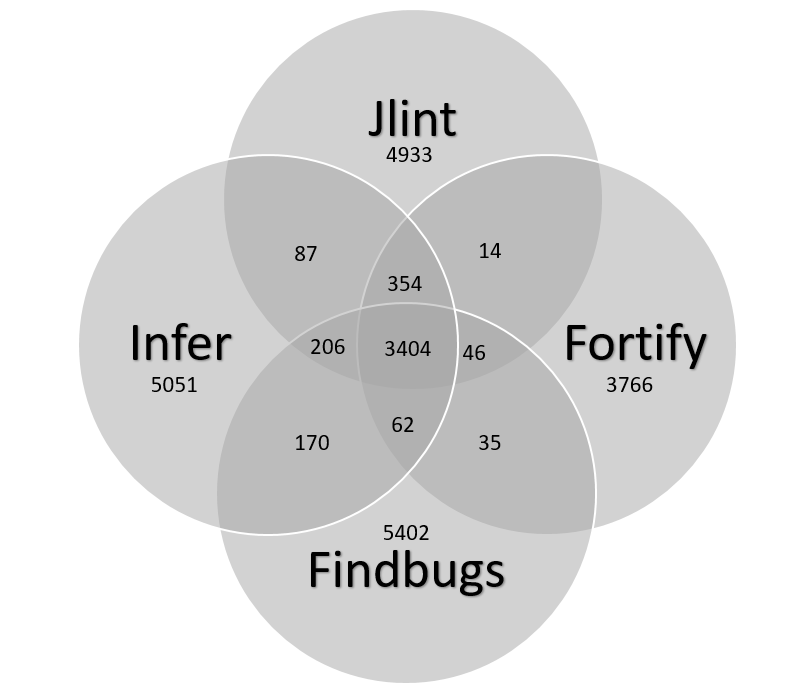
\includegraphics[width=0.70\textwidth]{figures/vnfigure3-1}
	\caption{4种工具在7429个测试用例上的检测结果}\label{fig:figure3-1}
\end{figure}

\begin{table}
	\centering
	\caption{四种工具和BIT-Detector的测试结果对比} \label{tab:table3-1}
	\begin{tabular*}{0.9\textwidth}{@{\extracolsep{\fill}}ccccc}
		\toprule
		测试工具	&正报	&误报	&准确率	&召回率 \\
		\midrule
		Findbugs	&5402	&3169	&63\%	&72\% \\
		Jlint	&4933	&9137	&35\%	&66\% \\
		Infer	&5051	&3578	&58\%	&68\% \\
		Fortify	&3766	&2211	&63\%	&50\% \\
		BIT-Detector	&3404	&576	&85\%	&45\% \\
		\bottomrule
	\end{tabular*}
\end{table}
\section{设计思路}
\section{整体架构}
\section{组织结构}
\section{本章小结}